% ----------------------------------------------------------------------
% 13eme Colloque National en Calcul des Structures
% ----------------------------------------------------------------------
% 15-19 mai 2017, Presqu'ile de Giens
% ----------------------------------------------------------------------
\documentclass{CSMA2017}
% ----------------------------------------------------------------------
\title{Méthodes de Newton non--lisses pour les problèmes de contact frottant dans les systèmes de multi--corps flexibles.}
% ----------------------------------------------------------------------
\author{V. Acary$^1$, M. Brémond$^2$, F. Dubois$^1$}
% ----------------------------------------------------------------------
\address{%
$^1$ INRIA. Grenoble, \{vincent.acary,maurice.bremond\}@inria.fr\\
$^2$ LMGC, Université de Montpellier, frederic.dubois@umontpellier.fr \\
}

% Mettre vos commandes personneles ici
% ----------------------------------------------------------------------
% Les commances \vect et \tens sont définies dans le fichier CSMA2017.cls




% ----------------------------------------------------------------------
\begin{document}
% ----------------------------------------------------------------------
\maketitle
% ----------------------------------------------------------------------

\begin{abstract}
Dans cette contribution, on se propose d'évaluer la performance des méthodes de Newton non--lisses dans le contexte des systèmes multi--corps flexibles (mécanismes, milieux granulaires ou milieux divisés) avec contact et frottement. Les méthodes itératives de type projection/relaxation (Jacobi ou Gauss--Seidel projeté) sont généralement utilisées pour leur propriétés de robustesse et de régularisation des systèmes fortement hyper--statiques. On montre que dans le cas des systèmes déformables, les méthodes de Newton permettent d'atteindre de grandes précisions a un coût beaucoup plus faible.

\keywords contact unilatéral, frottement de Coulomb, méthodes Newton non--lisses.
\end{abstract}

\section{Introduction}

Dans le contexte des systèmes multi--corps avec contact et frottement de Coulomb, le problème de contact frottant discret que l'on obtient a chaque pas de temps après une discrétisation temporelle, ou a chaque pas de chargement en quasi--statique, est généralement résolu par des méthodes itératives de type projection/relaxation (Jacobi ou Gauss--Seidel projeté). 
%
Pour les systèmes de corps rigides, qui sont pour la plupart fortement hyperstatique du fait d'un grand nombre de contacts en regard du nombre de degrés de liberté, les méthodes itératives jouissent de bonnes propriétés de robustesse. Elles permettent de converger de façon sure, mais lentement vers une solution du problème mais si les forces de réaction ne sont pas définies de manière unique. Il est connu que ces méthodes de Newton non--lisses sont totalement inopérantes pour les systèmes rigides hyperstatiques~\cite{bertailsdescoubes:inria-00557706, ??}.


Dans le cas de système de corps flexibles, discrétisés par exemple par des éléments finis, il est facile de réduire ce degré d'hyperstaticité en augmentant le nombre de degrés de liberté du système de façon à éviter les contraintes dépendantes au contact. Ceci peut par exemple se faire en raffinant les maillages a contact tout en contrôlant le nombre de point de contact générés.
%
Dans cette contribution, on montrer qu'il devient alors intéressant d'utiliser des méthodes de Newton non lisses pour résoudre le problème discret surtout si on veut atteindre des niveaux de précision relative supérieurs à $10^{-4}$.  Alors que les méthodes itératives de type projection/relaxation continuent à converger lentement, les méthodes de Newton retrouvent leurs convergences quadratiques locales pour des systèmes fortement réguliers. Cela permet d'atteindre des niveaux de précisions arbitraires pour un coût de calcul bien moindres. Dans ce travail, on essaye aussi de montrer qu'il peut être intéressant d'introduire \marginpar{voir si on peut le faire} un modèle de comportement élastique dans un système rigide afin de profiter des avantages d'un point de vue numériques des méthodes de Newton. Dans des travaux antérieurs, M. Jean~\cite{Jean1999,Acary.Jean98} avait montré que l'introduction de l'élasticité permettait de réduire le degré d'hyperstaticité et d'améliorer sensiblement la qualité des solutions en termes de forces de réaction. En préférant des méthodes de Newton non--lisses, on améliore aussi fortement le coût de calcul.




\begin{itemize}
\item Description du problème de frottement discret
\item Problème de rang de H
\item Objectifs du papier
  \begin{enumerate}
  \item Comparaison performance NSGS/NSN sur des déformables et des rigides.
  \item Intérêt a passer en déformable pour ajouter des ddl.
  \end{enumerate}
\end{itemize}

\section{Méthodes numériques de résolution}

\section{Profils de perfomance}

\section{Comparaison sur des solides élastiques}

\subsection{La murette}
\subsection{Résultats}
\begin{figure}
  \centering
  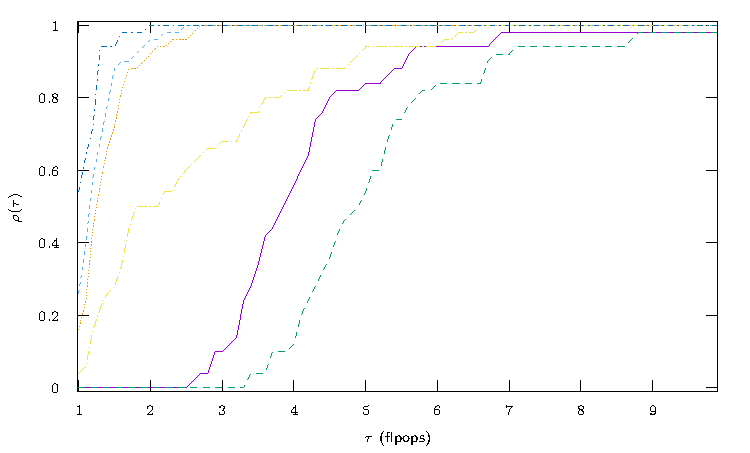
\includegraphics{figure/LowWall_FEM.1e-3.with_guess/simple/profile-LMGC_LowWall_FEM.pdf}
  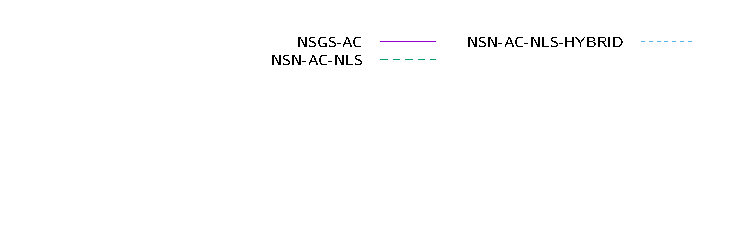
\includegraphics{figure/LowWall_FEM.1e-3.with_guess/simple/profile-LMGC_LowWall_FEM_legend.pdf}
  \caption{Comparaison entre le solveur NSGS-AC et NSN-AC pour une précision de $10^{-3}$}
  \label{fig:LowWall_FEM.1e-3.simple}
\end{figure}
\begin{figure}
  \centering
  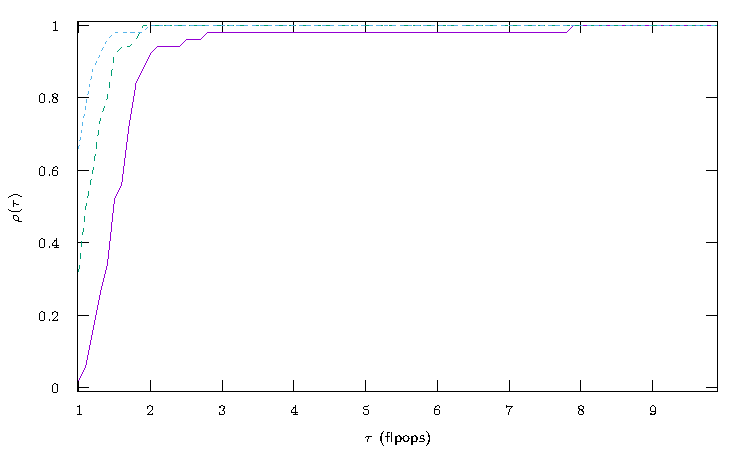
\includegraphics{figure/LowWall_FEM.1e-4.with_guess/simple/profile-LMGC_LowWall_FEM.pdf}
  \includegraphics{figure/LowWall_FEM.1e-4.with_guess/simple/profile-LMGC_LowWall_FEM_legend.pdf}
  \caption{Comparaison entre le solveur NSGS-AC et NSN-AC pour une précision de $10^{-4}$}
  \label{fig:LowWall_FEM.1e-4.simple}
\end{figure}
\begin{figure}
  \centering
  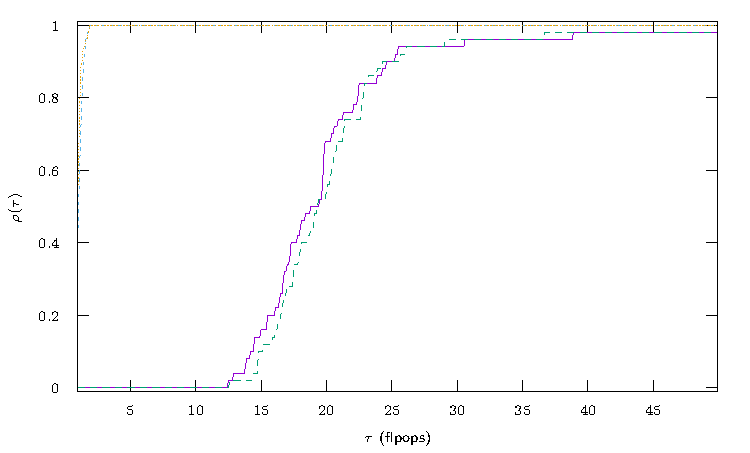
\includegraphics{figure/LowWall_FEM.1e-6.with_guess/simple/profile-LMGC_LowWall_FEM.pdf}
  \includegraphics{figure/LowWall_FEM.1e-6.with_guess/simple/profile-LMGC_LowWall_FEM_legend.pdf}
  \caption{Comparaison entre le solveur NSGS-AC et NSN-AC pour une précision de $10^{-6}$}
  \label{fig:LowWall_FEM.1e-6.simple}
\end{figure}


\begin{figure}
  \centering
  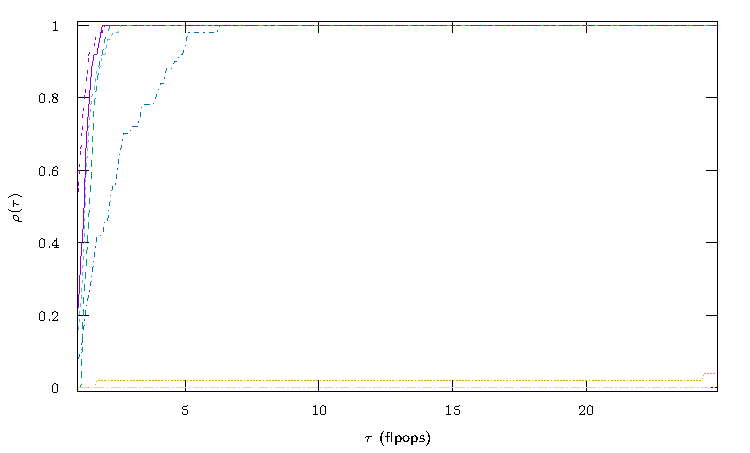
\includegraphics{figure/LowWall_FEM.1e-4.with_guess/nsn_nls/profile-LMGC_LowWall_FEM.pdf}
  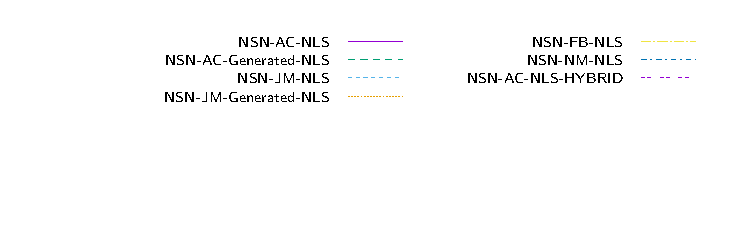
\includegraphics{figure/LowWall_FEM.1e-4.with_guess/nsn_nls/profile-LMGC_LowWall_FEM_legend.pdf}
  \caption{Comparaison des solveurs NSN-*-NLS pour une précision de $10^{-4}$}
  \label{fig:LowWall_FEM.1e-4.nsn_nls}
\end{figure}
\begin{figure}
  \centering
  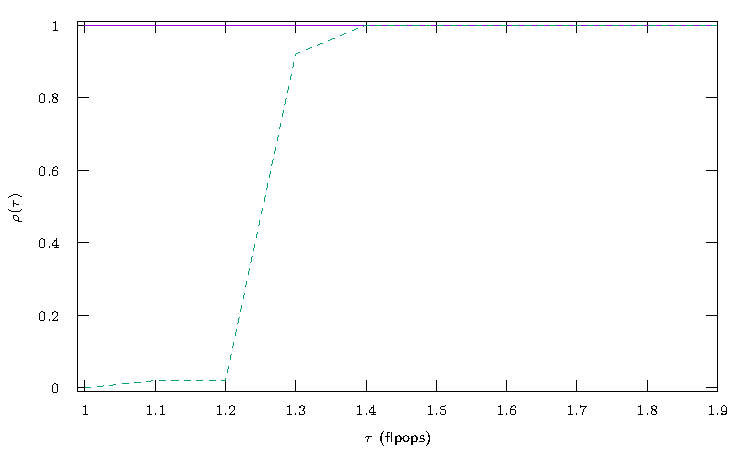
\includegraphics{figure/LowWall_FEM.1e-4.with_guess/nsgs/profile-LMGC_LowWall_FEM.pdf}
  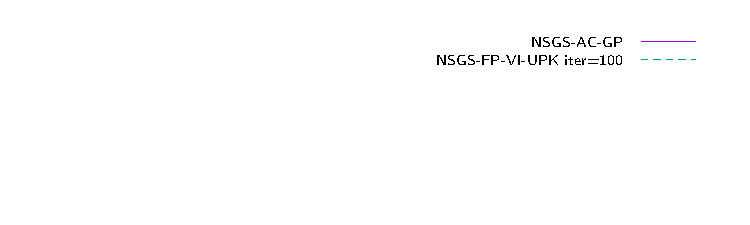
\includegraphics{figure/LowWall_FEM.1e-4.with_guess/nsgs/profile-LMGC_LowWall_FEM_legend.pdf}
  \caption{Comparaison des solveurs NSGS pour une précision de $10^{-4}$}
  \label{fig:LowWall_FEM.1e-4.nsgs}
\end{figure}

\section{Comparaison sur des solides rigides}

\section{Utilisation des solides élastiques pour améliorer la convergence}

\section{Conclusion}

parralelisme.
\subsection{Références bibliographiques}

% Les références sont à insérer en fin de document, numérotées par ordre alphabétique des auteurs. Trois exemples de références sont proposés : un article \cite{article} et un acte \cite{acte} et un livre  \cite{livre}.


\bibstyle{plain}

\bibliography{biblio}

% % ----------------------------------------------------------------------
% \begin{thebibliography}{1}
% % ----------------------------------------------------------------------
% \bibitem{article}
% P. Auteur, D. Auteur, T. Auteur. \emph{Titre de l'article}, Revue, Éditeur, page1-pageN, Année. 
% \bibitem{acte} P. Auteur. \emph{Titre de l'acte}, Titre de l'ouvrage, Éditeur, page1-pageN, Année.
% \bibitem{livre} P. Auteur, D. Auteur. \emph{Titre de l'ouvrage}, Éditeur, Année. 

% % ----------------------------------------------------------------------
% \end{thebibliography}
% % ----------------------------------------------------------------------

% ----------------------------------------------------------------------
\end{document}
% ----------------------------------------------------------------------
